\chapter{Logistika}

\section{Definice Logistiky}

Logistika zahrnuje všechny operace, které se týkají doručení zboží nebo služeb od výrobce k zákazníkovi, s výjimkou samotné výroby zboží nebo provádění služby. Výrobou je naopak rozuměno vše, co mění podobu materiálu.
Během výroby se však logistika uplatňuje, například jako přesun materiálu nebo polotovarů mezi jednotlivými výrobními zařízeními. 
% Obdobně při poskytování služby je podstatné se zabývat 
Operace lze rozdělit do tří hlavních toků: materiálový, informační a finanční tok. Materiálový obsahuje všechny pohyby týkající se fyzického materiálu, tedy jeho získávání, přesuny a skladování, a to jak mezi zákazníky, dodavateli či výrobními areály a sklady, tak i vnitřní pohyby mezi produkčními linkami nebo skladovými pozicemi. Informační tok popisuje procesy vznikající během materiálového toku, dále se do něj řadí analýzy již proběhlých toků a plánování a předpovědi budoucích toků. Poslední kategorie, finanční tok mapuje náklady způsobené předešlými dvěma zmíněnými toky.\cite{bib:Baudin}

Pojem logistika je úzce propojen s pojmem Supply Chain Management (SCM)\footnote{Do češtiny lze Supply Chain Management přeložit jako řízení či správa dodavatelského řetězce. V českém prostředí se používá jak anglická tak česká podoba.}. Zatímco logistika se zabývá toky zboží, služeb či lidí, Supply Chain Management zahrnuje operace logistiky, navíc ale sleduje vztahy mezi procesory, které koordinuje a optimalizuje za účelem naplnění určitých cílů. Tímto cílem bývá často snížení nákladů v rámci částí procesu nebo zvýšení konkurenceschopnosti podniku \cite{bib:IIMudaipur}. Supply Chain Management se tedy prolíná s pojmem logistika a bývají často zaměňovány. Důvodem může být i to, že se jedná o nový pojem, který byl poprvé použitý v roce 1982.\cite{bib:Christopher} 

\section{Štíhlá logistika}

Štíhlost neboli "lean" je koncept neustálého vylepšování procesu vytváření produktu nebo služby pomocí odstranění jakéhokoli plýtvání. Plýtváním rozumíme jakoukoli činnost, která v očích zákazníka nezvyšuje hodnotu produktu a tedy není ochotný za tuto činnost zaplatit ve formě vyšší prodejní ceny. Z této definice plýtvání je patrné, že pohled zákazníka hraje důležitou roli při vytváření hodnoty produktu ve štíhlých systémech.\cite{bib:LW1, LW2}

Svůj původ nachází štíhlá logistika na začátku 20. století, kdy henry Ford zavedl pohyblivou montážní linku při výrobě automobilu Ford modelu T. Tato linka měla za následek několikanásobné snížení výrobního času a odstartovala sériovou výrobu aut. Díky čemuž se snížila prodejní cena, a  automobily tak byly dostupné nejen nejbohatší vrstvě společnosti. 
Po druhé světové válce navázala automobilová společnost Toyota Motor Company na Fordovu efektivní montážní linku a vytvořila systém nazvaný Toyota Production System (TPS), který je přímým předchůdcem štíhlé logistiky.\cite{bib:seven}

\subsection{Toyota Production System}

Toyota Production System je založen na pěti základních principech. Nejdůležitějším krokem je odstranit plýtvání. Je třeba se soustředit na jednotlivé procesy a na vazby mezi nimi. Pomocí metody genchi genbutsu\footnote{Genchi v překladu znamená skutečná lokace a genbutsu skutečná věc.} se nasbírají data a informace o procesech přímo na místě, kde procesy probíhají, aby případné problémy a zdroje plýtvání mohly být přesně určeny. Po této analýze se aplikuje přístup řešení problémů zvaný kaizen\footnote{Kaizen je japonský překlad slova zlepšení.}, jehož cílem je kontinuální zlepšování procesů. Posledním z principů je  dodržování vzájemného respektu mezi všemi oddělení společnosti, jak vedoucími pracovníky, tak zaměstnanci u výrobních linek. \cite{bib:seven}

V TPS je plýtvání rozděleno do tří kategorií - Muda (plýtvání), Mura (nevyváženost) a Muri (přetěžování) \cite{bib:LW3}. V následující části jsou podrobněji popsány jednotlivé typy.

\subsubsection*{Muda}

Japonské označení Muda v překladu znamená plýtvání, neužitečnost či marnost. Muda zahrnuje všechny činnosti, které nepřispívají ke zvyšování hodnoty produktu. Mudu lze rozdělit na dva podtypy -- 1. typ zahrnuje aktivity, které jsou nezbytné pro koncového zákazníka, např. testování, zda je produkt nebo služba bezpečná. Druhý typ obsahuje ty procesy, které již zákazník nepotřebuje, či dokonce nechce, neboť mohou mít vliv na rychlost výroby produktu (výkonu služby) nebo přímo na jeho kvalitu.

Taiichi Ohno, manažer ve společnosti Toyota, identifikoval sedm typů plýtvání, někdy nazývané \emph{seven deadly wastes}. Klasifikace a popis včetně příkladů je uveden níže \cite{bib:seven}:
\begin{enumerate}
    \item \textbf{Nadprodukce} -- Pokud je vyrobeno více produktů, než je možné expedovat k zákazníkovi, nebo více materiálu, než kolik je požadováno k další výrobě či okamžité spotřebě.
    \item \textbf{Zpoždění/čekání} -- Jakákoli prodleva mezi dvěma na sebe navazujícími procesy, např. čekání jedné montážní linky na meziprodukty z jiné linky vlivem rozdílných výrobních časů nebo vlivem nedostatečné výrobní kapacita jednoho ze strojů, dále sem patří také čekání zaměstnanců z důvodu kontroly odvedené práce, pomalého načítání počítačového programu nebo čekání na konkrétní instrukce k výkonu práce \cite{bib:LW1}.
    \item \textbf{Transport} -- Zbytečný přesun produktů, materiálů nebo informací. Tento transport navíc může vést k poškození produktu. Příkladem tohoto typu plýtvání může být situace, kdy materiál, který je nejvíce potřebný pro výrobu produktů je umístěn v největší vzdálenosti, nebo pokud přístup k jedné položce ve skladu je blokovaný jinými položkami.
    \item \textbf{Pohyb} -- Zbytečný pohyb lidí, vzniklý špatným rozmístěním objektů v prostoru, např. nepřiměřeně dlouhotrvající chůze, natahování se pro předměty, vyhýbání se lidem či předmětům. 
    \item \textbf{Skladování} -- Pokud je naskladněno více surovin, rozpracovaných výrobků a hotových produktů, než kolik je požadováno, např. předčasná dovážka položek do skladu, chyba v dodávce, naskladnění položek do zásoby tzv. pro jistotu nebo z důvodu množstevní slevy.
    \item \textbf{Nadbytečné zpracování} -- Při výrobě dochází k použití více energie nebo prostředků než nutné, nebo je vytvořen koncový produkt, který má vyšší hodnotu, než jaký je dohodnutý a požadovaný standard. 
    \item \textbf{Defekty} -- Produkty či meziprodukty, které je nutné přepracovat nebo odstranit z výroby z důvodu vady. 
\end{enumerate}

Tyto podoby plýtvání aplikované v TPS byly inspirací pro identifikaci sedmi typů plýtvání v logistice \cite{bib:seven, bib:Jirsak}:
\begin{enumerate}
    \item \textbf{Nadprodukce} -- V případě logistiky je nadprodukce chápána jako doručení produktů dříve nebo ve větším množství něž bylo požadováno.
    \item \textbf{Zpoždění/čekání} -- Jakákoli prodleva mezi dvěma na sebe navazujícími procesy, např. čekání na převoz meziproduktů mezi dvěma výrobními linkami, příjezd kamionu mimo časové okno, doba mezi příjezdem kamionu a jeho naložením nebo čas mezi přijetím objednávky a zahájením její realizace. 
    \item \textbf{Transport} -- Zbytečný přesun produktů, materiálů nebo informací, např. materiál, který je nejvíce potřebný pro výrobu produktů je umístěn v největší vzdálenosti, nebo pokud přístup k jedné položce ve skladu je blokovaný jinými položkami.
    \item \textbf{Pohyb} -- Zbytečný pohyb lidí, např. vzniklý špatnou organizací předmětů ve skladu, kdy položky, ke kterým se nejčastěji přistupuje, jsou v méně přístupných pozicích skladu, nebo dokonce sklad není strukturovaný vůbec, nebo nutnost změnit trasu při převozu položek ve skladu kvůli nedostatečně širokým uličkám.
    \item \textbf{Skladování} -- Pokud je naskladněno více surovin, rozpracovaných výrobků a hotových produktů, než kolik je požadováno, např. předčasná dovážka položek do skladu, chyba v dodávce, naskladnění položek do zásoby tzv. pro jistotu.
    \item \textbf{Prostor} -- Neoptimální využití dostupného místa, např. nedostatečná výška regálů ve skladech, nevyužitá kapacita regálů, neoptimální naložení kamionu, přetížení dostupných kapacit.
    \item \textbf{Defekty} -- Činnosti, které způsobí nutnost opakovat určitý proces, znehodnocení produktu nebo zvýší náklady, např. špatné zavezení produktu, špatné nebo chybějící označení produktu, chyby v evidenci.
\end{enumerate}

V devadesátých letech, kdy se metody TPS začaly aplikovat ve společnostech, byl mezi sedm typů plýtvání Muda začleněn osmý typ - Dovednosti. V tomto případě dochází k neefektivitě kvůli nevyužití lidského potenciálu a talentů jednotlivých zaměstnanců. K tomu může docházet například striktním rozdělením na manažery a zaměstnance, kde role zaměstnanců je poslouchat nařízení shora a vykonávat práci tak, jak byla navržena vedoucími pracovníky. Avšak právě zaměstnanci pracující přímo v terénu lépe identifikují případné problémy a snadněji naleznou řešení díky svým zkušenostem.\cite{bib:LW1}


% Základním kamenem pro odstranění plýtvání v TPS je koncept "Just-in-Time", při jehož aplikování se vyrábí pouze to, co je aktuálně potřeba v přesně požadovaném množství.

\subsubsection*{Mura}

Mura lze přeložit jako nestejnoměrnost, nevyrovnanost a nepravidelnost. Jedná se o plýtvání vznikající špatnou provázaností jednotlivých procesů a to jak interních, tak externích. Následkem nevyváženosti je pak vznik plýtvání Muda. \cite{bib:LW3, bib:Jirsak}

Plýtvání v podobě Mura se rozlišuje jak v procesech informačního, tak hmotného toku. V případě informačního toku je nejvýznamnějším zdrojem plýtvání situace, 
kdy je chybně predikována poptávka mezi jednotlivými články logistického řetězce. Ignorování vztahů mezi procesy může vést k chybovosti i v řádu desítek procent. Informace, jejichž opomíjeni způsobuje chybovost předpovídání poptávky, mohou být např. v jaké fázi životního cyklu se výrobek nachází, plánování promoakcí nebo výrobní a logistická omezeni dodavatelů.
Další zdroj Mura v informačním toku je nedostatečná znalost stavu zásob mezi dodavatelem a odběratelem. Následkem čehož dochází k méně častým zavážkám avšak s větším objemem, což vede k vyšším pojistným zásobám ve skladech. Většinu zmíněných situací lze eliminovat aplikováním konceptu "Just-in-Time" do jednotlivých procesů.
Plýtvání také vzniká při administrativě, pokud nejsou vhodně standardizované dokumenty používané v logistickém řetězci. Příkladem může být špatná evidence pohybů ve skladu či tvorba objednávek. Nesjednocenost v administrativních procesech vede ke zpomalení navazujících činností nebo dokonce k chybám, které způsobí nemožnost dokončení celého procesu. Pak je nutné vybrané procesy provést znovu a napravit chyby.\cite{bib:Jirsak}

Plýtvání v hmotném toku je přímým důsledkem chyb vznikajících v informačním toku. Lze identifikovat i takové zdroje plýtvání, které nesouvisejí přímo s informačním tokem, a to například dodržování různých standardů přepravních prostředků na straně dodavatele a odběratele. To má pak za následek nadbytečné překládání materiálu do podoby, kterou druhá strana používá a se kterou je schopna následně efektivněji manipulovat.\cite{bib:Jirsak}

\subsubsection*{Muri}

Pojem Muri označuje přetěžování. Muri často vzniká při snaze zvýšit produktivitu a odstranit tak předešlé typy plýtvání, v konečném důsledku může ale vést k výrazně větší chybovosti i celkovému selhání. Přetíženi mohou být zaměstnanci, ale i stroje. V obou případech vytížení na více než 100 \% se může projevit na snížení kvality výstupu.  Lidé mohou být méně pozorní a může docházet k nehodám, které mohou v menší či větší míře negativně ovlivnit i větší část logistického řetězce. Stroje mohou produkovat zmetkové výrobky, nebo může dojít k jejich poškození až zničení.\cite{bib:Jirsak,bib:LW3}

\subsubsection*{Příklad plýtvání Muda, Mura a Mudi}

Všechny tři zmíněné typy plýtvání Muda, Mura a Muri jsou navzájem propojené. Tuto skutečnost je třeba brát v potaz při řešení zefektivňování procesů a eliminaci plýtvání. Pro představu je uvedena následující situace. Společnost potřebuje zákazníkovi přivézt šest tun materiálu, uloženého ve stejných jednotunových kontejnerech. Možné způsoby řešení této úlohy jsou znázorněné na obr. \ref{obr:log:3M}.\cite{bib:LW3}

\begin{figure}[h!]
    \centering
    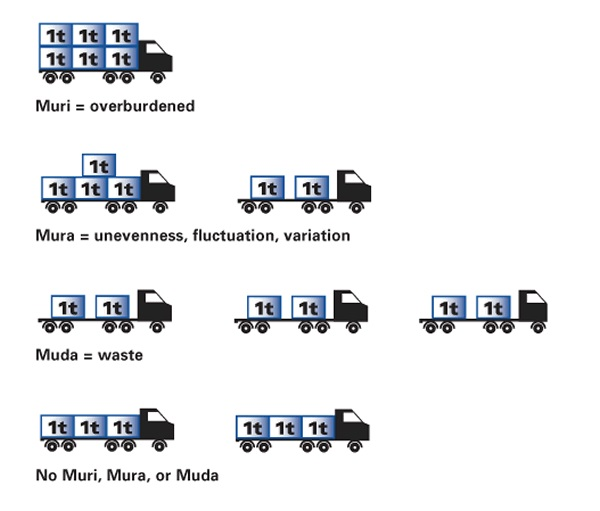
\includegraphics[width=0.9\textwidth]{obrazky/3M.jpg}
    \caption{Příklady plýtvání Muda, Mura a Muri při transportu šesti tun materiálu.\cite{bib:LW3}}
    \label{obr:log:3M}
\end{figure}

Nejjednodušší možností je naložit na jeden kamion veškerý požadovaný materiál. V takovém případě společnost ušetří na počtu vozidel a eliminuje tak plýtvání přepravními prostředky, ušetří čas při nakládce a vykládce, protože není nutné obsluhovat více vozidel, zároveň . Na druhou stranu ale hrozí přetížení kamionu. Následkem přetížení se může zvýšit riziko nehody vozidla, firma může být pokutována nebo vozidlu nemusí být umožněn vjezd na určitá místa.

Opačným extrémem je použít tři kamiony, každý se dvěma tunami materiálu. Potom ale není efektivně využita dostupná kapacita a je patrné, že dochází k mnoha druhům plýtvání typu Muda.

Třetí možností je využití dvou kamionů, kdy první je naložen čtyřmi a druhý dvěma tunami. Toto rozložení nepodléhá žádným pravidlům a patrně proces nakládky není dostatečně spjatý s ostatními procesy nebo neprobíhá správný přenos informací o požadavcích mezi jednotlivými procesy. Nakládka a vykládka prvního velmi naloženého kamionu vyžaduje více času než druhého kamionu. Z toho plyne, že buď není možné v dostupném čase stihnout obsloužit první kamion a dochází k přetížení, anebo v případě druhého kamionu je zbude velké množství času a zaměstnanci zbytečně čekají. Z této volby plyne, že plýtvání typu Mura může způsobit Mudu i Muru.\cite{bib:LW3}

Optimální řešení je naložit dva kamiony po třech tunách, což je jejich ideální kapacita. V takovém případě společnost minimalizuje za daných podmínek všechny tři typy plýtvání. V reálném světě jsou situace mnohonásobně komplexnější a ne vždy existuje jednoznačné optimální řešení, které je navíc snadno dosažitelné. Důležité ale je soustředit se na všechny tři typy současně, protože optimalizace pouze jednoho kritéria může způsobit jiný druh plýtvání nebo kolaps části systému. 

V roce 2011 bylo realizováno dotazníkové šetření Vysokou školou ekonomickou v Praze, které mapovalo, kolik procent logistických expertů se zabývá odstraněním zmiňovaných tří typů plýtvání. Plýtvání Muda se snaží odstranit z logistických procesů 72 \% respondentů, Murou se zabývá 39 \% a plýtvání Muri řeší 30 \% dotazovaných.\cite{bib:Jirsak}

\subsection{Plýtvání v logistických procesech}

Tato sekce se zabývá třinácti vybranými logistickými procesy z hlediska plýtvání, jak jsou uvedeny v knize \emph{Logistika pro ekonomy -- Vstupní logistika}. Analýza vychází z již zmíněného dotazníkového šetření z roku 2011.